%!TEX TS-program = xelatex
\documentclass[main]{subfiles}
%这是一个子文件,单独编译时会自动导入main文件的导言区
%这里可以放自定义命令,不会和别人的冲突请放心
%但是不能放newtheorem等高级命令,需要请在群里说
%下面是一些数学命令的简化,可以保留,可以删去,也可以按你的习惯修改
\def\e{\textup{e}}
\def\i{\textup{i}}
\def\T{\textup{T}}
\def\diag{\textup{diag}}
\def\id{\textup{id}}
\newcommand{\toi}[1]{{#1}\to\infty}
\newcommand{\dis}{\displaystyle}
\newcommand{\bv}{\mathrm{BV}}
\newcommand{\ac}{\mathrm{AC}}
\newcommand{\mr}{\mathbb{R}}
\newcommand{\mn}{\mathbb{N}}
\newcommand{\mq}{\mathbb{Q}}
\newcommand{\mz}{\mathbb{Z}}
\newcommand{\rel}{\text{ rel }}
\newcommand{\sgn}{\operatorname{sign}}
\newcommand{\ve}{\varepsilon}
\newcommand{\bs}{\backslash}
\renewcommand{\ll}{\lim\limits}
\renewcommand{\span}{\operatorname{span}}
\renewcommand{\ker}{\operatorname{Ker}}
\renewcommand{\hom}{\operatorname{Hom}}
\renewcommand{\leq}{\leqslant}
\renewcommand{\geq}{\geqslant}
\begin{document}
\renewcommand{\filename}{subfile7}%在这里填你的文件名,避免\label冲突
%这里开始写你的代码
%\title{subfile7}\renewcommand\maketitlehookc{\vspace{-18ex}}\date{}
%\maketitle
\captionsetup[figure]{name={图},labelsep=period} 
\section{Euler的多面体公式 $V-E+F=2$}
\subsection{背景介绍}
对于一个简单多面体(表面能同胚于一个球面的多面体), 记它的\textbf{顶点(vertex)}数为$V$, \textbf{棱(edge)}数为$E$, 
\textbf{面(face)}数为$F$, 则这三个量满足公式$V-E+F=2$, 即Euler多面体公式(Euler's Polyhedron Formula). 这一公式早在1639年被Descartes注意到并证明;
通过Descartes的手稿, Leibniz 1675年也知道这个公式; 1750年, Euler 独立证明并发表了这个公式.


后来, Poincaré认识到Euler多面体公式的推广是典型的拓扑性质的
定理, 即$V-E+F=\chi$, 其中$\chi$为\textbf{Euler示性数(Euler characteristic)}, 是一个拓扑不变量; 例如上述球面(sphere)有$\chi=2$, 而环面(torus)有$\chi=0$.
这确立了Euler公式在拓扑学中的重要地位. 
\subsection{证明概述}
\begin{theorem}(Euler的多面体公式)
  对于简单多面体, 有公式$V-E+F=2$.
\end{theorem}
在这里,我们给出Cauchy在1811年提出的一种证明方法. 
勒让德利用球面三角学给出了证明; Descartes在他的手稿中也给出了证明, 用到了球面上多边形的立体角和它的平面角之间的关系. 后两种证明请阅读\textbf{王敬赓《直观拓扑》}p18\&p21
\begin{proof}
  任取球面上一点, 去掉该点任意一个闭邻域, 得到的图形同胚于一个平面; 由于简单多面体同胚于球面, 故
  去掉任意一个面的简单多面体可以在给定平面上展开成\textbf{平面图(各边互不交叠)}. 以正方体为例, 如图1所示, 
  这里正方体\ref{fig:subfig1}去掉了面EFGH, 展开成为平面图\ref{fig:subfig2}.

  \begin{figure}[h]    
      \centering            
      \subfloat []
      {
          \label{fig:subfig1}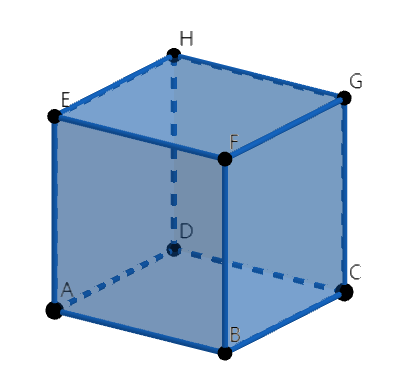
\includegraphics[width=0.2\textwidth]{cubic.png}
      }
      \subfloat[]
      {
          \label{fig:subfig2}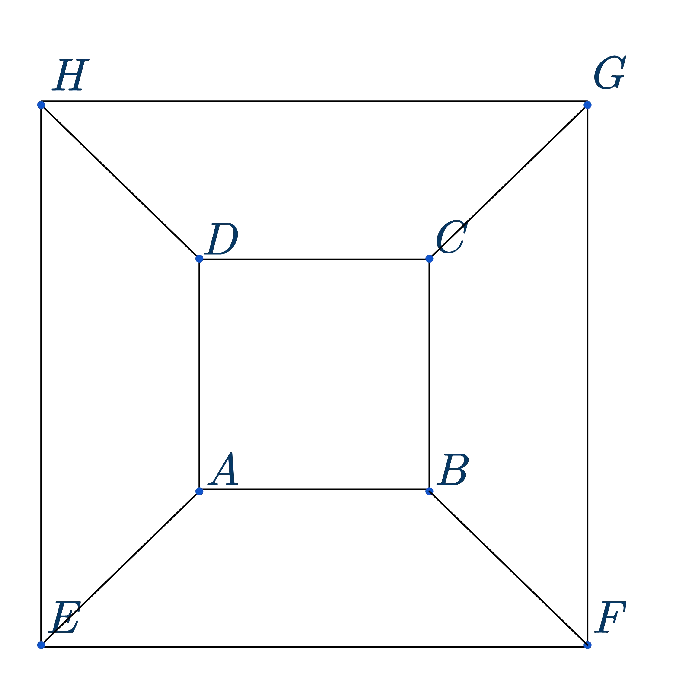
\includegraphics[width=0.18\textwidth]{plane1.pdf}
      }
      \subfloat[]
    {
        \label{fig:subfig3}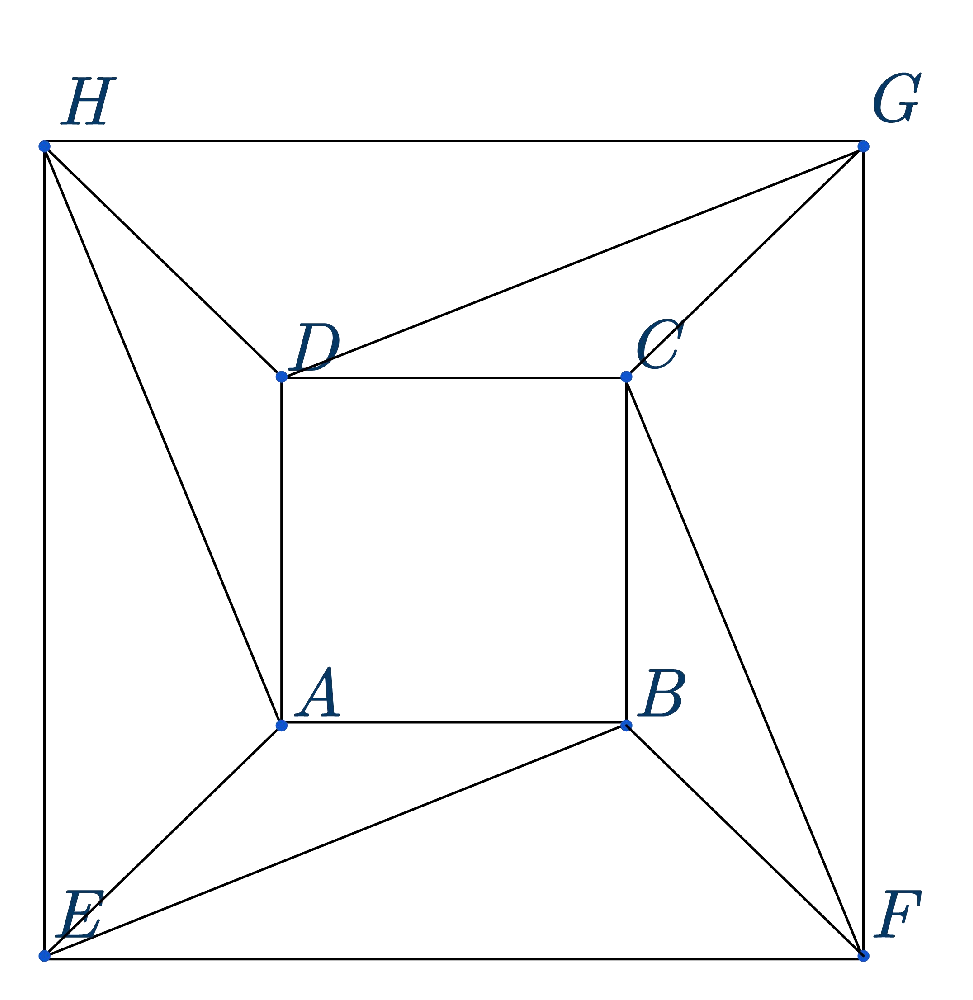
\includegraphics[width=0.18\textwidth]{plane2.pdf}
    }
    \subfloat[]
    {
        \label{fig:subfig4}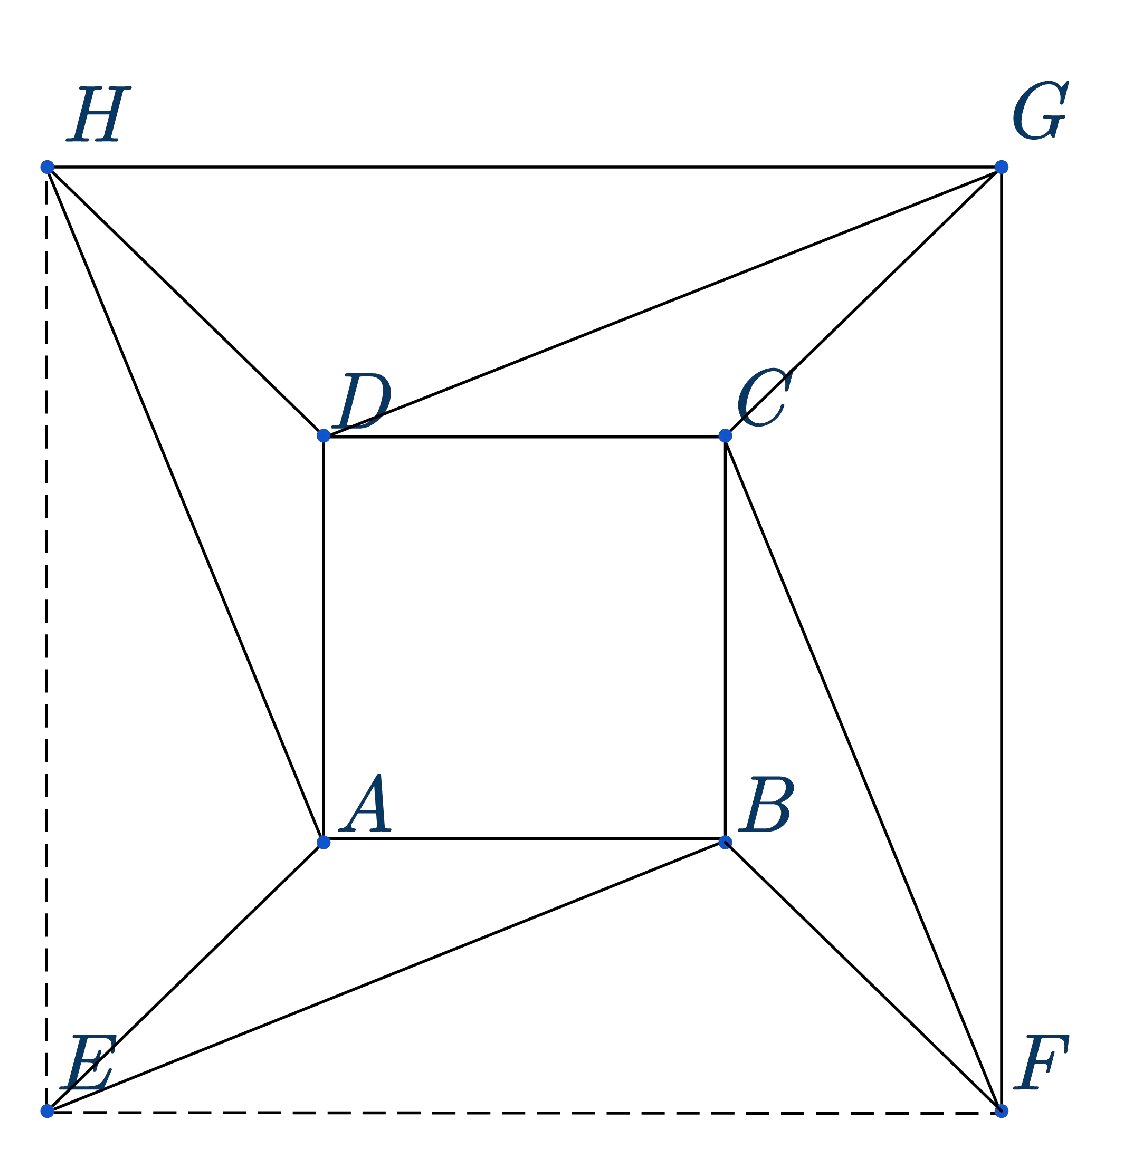
\includegraphics[width=0.18\textwidth]{plane3.pdf}
    }
    \subfloat[]
    {
        \label{fig:subfig5}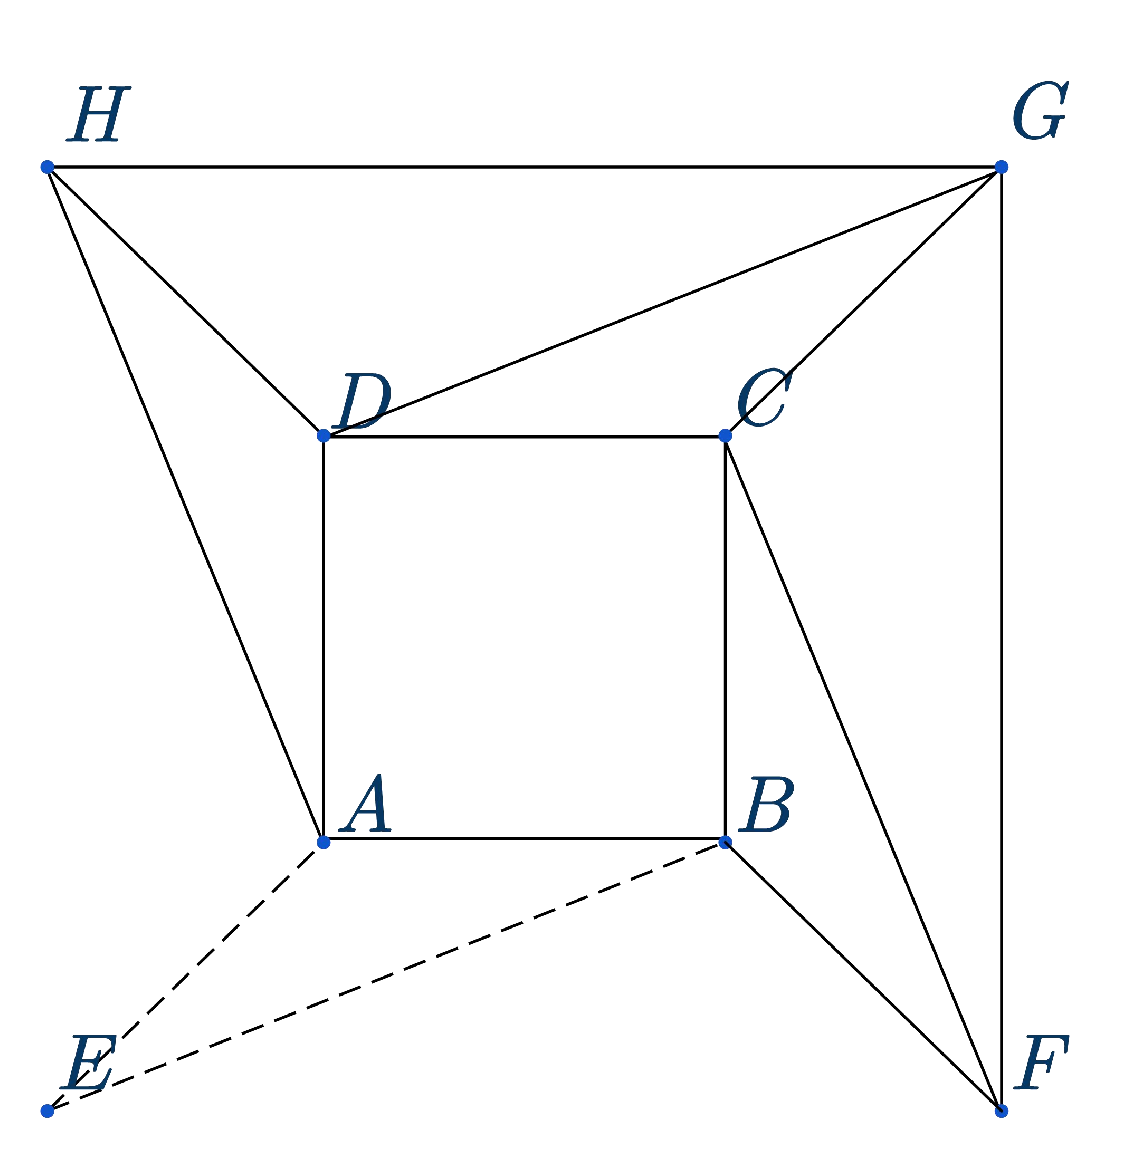
\includegraphics[width=0.18\textwidth]{plane4.pdf}
    }
      \caption{以正方体为例的操作流程}
      \label{fig:subfig_1} 
  \end{figure}

由于只去掉了一个面, 证多面体的Euler公式等价于证平面图的Euler公式\(V-E+F=1\).
我们接着对平面图做以下操作: 对于平面图里顶点数不是3的面, 在保持图是平面图的前提下, 
向这个面添加\textbf{边(edge)}(比如从给定顶点出发,向在同个面内的所有其他顶点连线); 我们对所有的面做这样的操作, 最后得到了一个每个面只有3个顶点的平面图,如图\ref{fig:subfig3}.

接着从最外围的面开始(至少有1条边不与其他面相邻), 如果这个面只有1条边不与其它面相邻, 去掉这条边,如图\ref{fig:subfig4}; 如果这个面有2条边不与其他面相邻, 同时去掉这2条边,如图\ref{fig:subfig5}.

我们重复上述操作, 最终得到一个三角形平面图, 这个图$V=3$, $E=3$, $F=1$, 满足$V-E+F=1$. 由于所有关于平面图的
操作均保持$V-E+F$不变, 故原来的关于平面图的等式也成立, 至此Euler的多面体公式得证.
\end{proof}

\subsection{应用}
1. 得到不可平面图的必要条件;2. 证明正多面体只有五种.\quad 参考: 王敬赓《直观拓扑》
\end{document}
